  \documentclass[msc,numbers]{coppe}

%Added by @MyKo101, code provided by @GerbrichFerdinands
\newlength{\cslhangindent}
\setlength{\cslhangindent}{1.5em}
\newenvironment{cslreferences}%
  {\setlength{\parindent}{0pt}%
  \everypar{\setlength{\hangindent}{\cslhangindent}}\ignorespaces}%
  {\par}

\usepackage{amsmath,amssymb}
\usepackage{hyperref}
\usepackage{longtable}
\usepackage{booktabs}

\providecommand{\tightlist}{%
  \setlength{\itemsep}{0pt}\setlength{\parskip}{0pt}}

\makelosymbols
\makeloabbreviations

\usepackage{color}
\usepackage{fancyvrb}
\newcommand{\VerbBar}{|}
\newcommand{\VERB}{\Verb[commandchars=\\\{\}]}
\DefineVerbatimEnvironment{Highlighting}{Verbatim}{commandchars=\\\{\}}
% Add ',fontsize=\small' for more characters per line
\usepackage{framed}
\definecolor{shadecolor}{RGB}{248,248,248}
\newenvironment{Shaded}{\begin{snugshade}}{\end{snugshade}}
\newcommand{\AlertTok}[1]{\textcolor[rgb]{0.94,0.16,0.16}{#1}}
\newcommand{\AnnotationTok}[1]{\textcolor[rgb]{0.56,0.35,0.01}{\textbf{\textit{#1}}}}
\newcommand{\AttributeTok}[1]{\textcolor[rgb]{0.77,0.63,0.00}{#1}}
\newcommand{\BaseNTok}[1]{\textcolor[rgb]{0.00,0.00,0.81}{#1}}
\newcommand{\BuiltInTok}[1]{#1}
\newcommand{\CharTok}[1]{\textcolor[rgb]{0.31,0.60,0.02}{#1}}
\newcommand{\CommentTok}[1]{\textcolor[rgb]{0.56,0.35,0.01}{\textit{#1}}}
\newcommand{\CommentVarTok}[1]{\textcolor[rgb]{0.56,0.35,0.01}{\textbf{\textit{#1}}}}
\newcommand{\ConstantTok}[1]{\textcolor[rgb]{0.00,0.00,0.00}{#1}}
\newcommand{\ControlFlowTok}[1]{\textcolor[rgb]{0.13,0.29,0.53}{\textbf{#1}}}
\newcommand{\DataTypeTok}[1]{\textcolor[rgb]{0.13,0.29,0.53}{#1}}
\newcommand{\DecValTok}[1]{\textcolor[rgb]{0.00,0.00,0.81}{#1}}
\newcommand{\DocumentationTok}[1]{\textcolor[rgb]{0.56,0.35,0.01}{\textbf{\textit{#1}}}}
\newcommand{\ErrorTok}[1]{\textcolor[rgb]{0.64,0.00,0.00}{\textbf{#1}}}
\newcommand{\ExtensionTok}[1]{#1}
\newcommand{\FloatTok}[1]{\textcolor[rgb]{0.00,0.00,0.81}{#1}}
\newcommand{\FunctionTok}[1]{\textcolor[rgb]{0.00,0.00,0.00}{#1}}
\newcommand{\ImportTok}[1]{#1}
\newcommand{\InformationTok}[1]{\textcolor[rgb]{0.56,0.35,0.01}{\textbf{\textit{#1}}}}
\newcommand{\KeywordTok}[1]{\textcolor[rgb]{0.13,0.29,0.53}{\textbf{#1}}}
\newcommand{\NormalTok}[1]{#1}
\newcommand{\OperatorTok}[1]{\textcolor[rgb]{0.81,0.36,0.00}{\textbf{#1}}}
\newcommand{\OtherTok}[1]{\textcolor[rgb]{0.56,0.35,0.01}{#1}}
\newcommand{\PreprocessorTok}[1]{\textcolor[rgb]{0.56,0.35,0.01}{\textit{#1}}}
\newcommand{\RegionMarkerTok}[1]{#1}
\newcommand{\SpecialCharTok}[1]{\textcolor[rgb]{0.00,0.00,0.00}{#1}}
\newcommand{\SpecialStringTok}[1]{\textcolor[rgb]{0.31,0.60,0.02}{#1}}
\newcommand{\StringTok}[1]{\textcolor[rgb]{0.31,0.60,0.02}{#1}}
\newcommand{\VariableTok}[1]{\textcolor[rgb]{0.00,0.00,0.00}{#1}}
\newcommand{\VerbatimStringTok}[1]{\textcolor[rgb]{0.31,0.60,0.02}{#1}}
\newcommand{\WarningTok}[1]{\textcolor[rgb]{0.56,0.35,0.01}{\textbf{\textit{#1}}}}
\begin{document}

  \title{Titulo de Tese}
  \foreigntitle{Thesis' Title}
    \author{Jefferson}{Silvério}
      \advisor{Prof.}{Gisele}{A. Oda}{D.Sc.}
    \advisor{Prof.}{Verónica}{Valentinuzzi}{Ph.D}
    \advisor{Prof.}{Patricia}{Tachinardi}{Ph.D}
  

    \examiner{Prof.}{Nome Completo do Primeiro Examinador}{D.Sc.}
    \examiner{Prof.}{Nome Completo do Segundo Examinador}{Ph.D}
    \examiner{Prof.}{Nome Completo do Terceiro Examinador}{Ph.D}
    \department{IB}
  \date{09}{2020}
    \keyword{Primeira palavra-chave}
    \keyword{Segunda palavra-chave}
    
  % Adiciona Pagina de Titulo
  \maketitle

  % Adiciona Pagina de Rosto com 
  \frontmatter
  
  %Adiciona dedicatorias
  \dedication{A alguém cujo valor é digno desta dedicatória.}
    \chapter*{Agradecimentos}
  Gostaria de agradecer a X
  
  % Adiciona Abstracts
  \begin{abstract}
  Sit urna lacus aenean euismod morbi integer mauris ligula euismod. Massa leo nunc rutrum non vulputate viverra erat aliquet torquent. Dictumst inceptos litora diam dui eu non sodales eget metus? Mollis faucibus justo class class nulla vestibulum consequat purus.

  Sit est ligula massa massa. Lectus parturient vehicula luctus nisl facilisis iaculis sagittis euismod ornare ut platea! Vestibulum et cras nostra luctus morbi cubilia et ante ornare luctus commodo facilisis nam. Lobortis ligula dictum tortor facilisis ante gravida habitasse cras laoreet. Vehicula pharetra vulputate non magna ut interdum habitant quam et class elementum arcu!

  Adipiscing nulla laoreet magna dignissim nostra phasellus lacinia elementum est id! Rutrum arcu aliquet torquent porttitor ligula eget dictumst aenean. Lacus dictumst phasellus sed lobortis leo convallis velit mi imperdiet. Ultricies convallis id vestibulum morbi rutrum tortor diam volutpat euismod montes enim cras eros luctus duis rutrum integer.

  Consectetur platea augue vitae vitae integer ad tincidunt torquent ac. Pharetra malesuada odio non lobortis dis aliquet arcu nascetur magna porttitor. Lacinia curabitur primis ligula magna sociosqu hendrerit sociosqu risus cubilia. Arcu potenti mi pellentesque nulla per varius vitae lectus pellentesque! Tempor.
  \end{abstract}
  \pagebreak
  \begin{foreignabstract}
  Sit urna lacus aenean euismod morbi integer mauris ligula euismod. Massa leo nunc rutrum non vulputate viverra erat aliquet torquent. Dictumst inceptos litora diam dui eu non sodales eget metus? Mollis faucibus justo class class nulla vestibulum consequat purus.

  Sit est ligula massa massa. Lectus parturient vehicula luctus nisl facilisis iaculis sagittis euismod ornare ut platea! Vestibulum et cras nostra luctus morbi cubilia et ante ornare luctus commodo facilisis nam. Lobortis ligula dictum tortor facilisis ante gravida habitasse cras laoreet. Vehicula pharetra vulputate non magna ut interdum habitant quam et class elementum arcu!

  Adipiscing nulla laoreet magna dignissim nostra phasellus lacinia elementum est id! Rutrum arcu aliquet torquent porttitor ligula eget dictumst aenean. Lacus dictumst phasellus sed lobortis leo convallis velit mi imperdiet. Ultricies convallis id vestibulum morbi rutrum tortor diam volutpat euismod montes enim cras eros luctus duis rutrum integer.

  Consectetur platea augue vitae vitae integer ad tincidunt torquent ac. Pharetra malesuada odio non lobortis dis aliquet arcu nascetur magna porttitor. Lacinia curabitur primis ligula magna sociosqu hendrerit sociosqu risus cubilia. Arcu potenti mi pellentesque nulla per varius vitae lectus pellentesque! Tempor.
  \end{foreignabstract}
  % Adiciona Sumário
  \tableofcontents
  
  % Adiciona Lista de Figuras
    \listoffigures
  
  % Adiciona Lista de Tabelas
    \listoftables
  
  % Adiciona Lista de Simbolos e Abreviacoes
  \printlosymbols
  \printloabbreviations

  % Adiciona Corpo da Tese
  \mainmatter
  \hypertarget{introduction}{%
  \chapter*{Introduction}\label{introduction}}
  \addcontentsline{toc}{chapter}{Introduction}

  Welcome to the \emph{R Markdown} thesis template. This template is based on (and in many places copied directly from) the Reed College LaTeX template, but hopefully it will provide a nicer interface for those that have never used TeX or LaTeX before. Using \emph{R Markdown} will also allow you to easily keep track of your analyses in \textbf{R} chunks of code, with the resulting plots and output included as well. The hope is this \emph{R Markdown} template gets you in the habit of doing reproducible research, which benefits you long-term as a researcher, but also will greatly help anyone that is trying to reproduce or build onto your results down the road.

  Hopefully, you won't have much of a learning period to go through and you will reap the benefits of a nicely formatted thesis. The use of LaTeX in combination with \emph{Markdown} is more consistent than the output of a word processor, much less prone to corruption or crashing, and the resulting file is smaller than a Word file. While you may have never had problems using Word in the past, your thesis is likely going to be about twice as large and complex as anything you've written before, taxing Word's capabilities. After working with \emph{Markdown} and \textbf{R} together for a few weeks, we are confident this will be your reporting style of choice going forward.

  \textbf{Why use it?}

  \emph{R Markdown} creates a simple and straightforward way to interface with the beauty of LaTeX. Packages have been written in \textbf{R} to work directly with LaTeX to produce nicely formatting tables and paragraphs. In addition to creating a user friendly interface to LaTeX, \emph{R Markdown} also allows you to read in your data, to analyze it and to visualize it using \textbf{R} functions, and also to provide the documentation and commentary on the results of your project. Further, it allows for \textbf{R} results to be passed inline to the commentary of your results. You'll see more on this later.

  \textbf{Who should use it?}

  Anyone who needs to use data analysis, math, tables, a lot of figures, complex cross-references, or who just cares about the final appearance of their document should use \emph{R Markdown}. Of particular use should be anyone in the sciences, but the user-friendly nature of \emph{Markdown} and its ability to keep track of and easily include figures, automatically generate a table of contents, index, references, table of figures, etc. should make it of great benefit to nearly anyone writing a thesis project.

  \textbf{For additional help with bookdown}
  Please visit \href{https://bookdown.org/yihui/bookdown/}{the free online bookdown reference guide}.

  \hypertarget{rmd-basics}{%
  \chapter{R Markdown Basics}\label{rmd-basics}}

  Here is a brief introduction into using \emph{R Markdown}. \emph{Markdown} is a simple formatting syntax for authoring HTML, PDF, and MS Word documents. \emph{R Markdown} provides the flexibility of \emph{Markdown} with the implementation of \textbf{R} input and output. For more details on using \emph{R Markdown} see \url{http://rmarkdown.rstudio.com}.

  Be careful with your spacing in \emph{Markdown} documents. While whitespace largely is ignored, it does at times give \emph{Markdown} signals as to how to proceed. As a habit, try to keep everything left aligned whenever possible, especially as you type a new paragraph. In other words, there is no need to indent basic text in the Rmd document (in fact, it might cause your text to do funny things if you do).

  Let's cite (Abraham, Marsden, and Ratiu \protect\hyperlink{ref-book-example}{1988}).

  \hypertarget{lists}{%
  \section{Lists}\label{lists}}

  It's easy to create a list. It can be unordered like
  \begin{itemize}
  \tightlist
  \item
    Item 1
  \item
    Item 2
  \end{itemize}
  or it can be ordered like
  \begin{enumerate}
  \def\labelenumi{\arabic{enumi}.}
  \tightlist
  \item
    Item 1
  \item
    Item 2
  \end{enumerate}
  Notice that I intentionally mislabeled Item 2 as number 4. \emph{Markdown} automatically figures this out! You can put any numbers in the list and it will create the list. Check it out below.

  To create a sublist, just indent the values a bit (at least four spaces or a tab). (Here's one case where indentation is key!)
  \begin{enumerate}
  \def\labelenumi{\arabic{enumi}.}
  \tightlist
  \item
    Item 1
  \item
    Item 2
  \item
    Item 3
    \begin{itemize}
    \tightlist
    \item
      Item 3a
    \item
      Item 3b
    \end{itemize}
  \end{enumerate}
  \hypertarget{line-breaks}{%
  \section{Line breaks}\label{line-breaks}}

  Make sure to add white space between lines if you'd like to start a new paragraph. Look at what happens below in the outputted document if you don't:

  Here is the first sentence. Here is another sentence. Here is the last sentence to end the paragraph.
  This should be a new paragraph.

  \emph{Now for the correct way:}

  Here is the first sentence. Here is another sentence. Here is the last sentence to end the paragraph.

  This should be a new paragraph.

  \hypertarget{r-chunks}{%
  \section{R chunks}\label{r-chunks}}

  When you click the \textbf{Knit} button above a document will be generated that includes both content as well as the output of any embedded \textbf{R} code chunks within the document. You can embed an \textbf{R} code chunk like this (\texttt{cars} is a built-in \textbf{R} dataset):
\begin{Shaded}
\begin{Highlighting}[]
\KeywordTok{summary}\NormalTok{(cars)}
\end{Highlighting}
\end{Shaded}
\begin{verbatim}
     speed           dist       
 Min.   : 4.0   Min.   :  2.00  
 1st Qu.:12.0   1st Qu.: 26.00  
 Median :15.0   Median : 36.00  
 Mean   :15.4   Mean   : 42.98  
 3rd Qu.:19.0   3rd Qu.: 56.00  
 Max.   :25.0   Max.   :120.00  
\end{verbatim}
  \hypertarget{inline-code}{%
  \section{Inline code}\label{inline-code}}

  If you'd like to put the results of your analysis directly into your discussion, add inline code like this:

  The \texttt{cos} of \(2 \pi\) is 1.

  Another example would be the direct calculation of the standard deviation:
  \begin{quote}
  The standard deviation of \texttt{speed} in \texttt{cars} is 5.2876444.
  \end{quote}
  One last neat feature is the use of the \texttt{ifelse} conditional statement which can be used to output text depending on the result of an \textbf{R} calculation:
  \begin{quote}
  The standard deviation is less than 6.
  \end{quote}
  Note the use of \texttt{\textgreater{}} here, which signifies a quotation environment that will be indented.

  As you see with \texttt{\$2\ \textbackslash{}pi\$} above, mathematics can be added by surrounding the mathematical text with dollar signs. More examples of this are in {[}Mathematics and Science{]} if you uncomment the code in {[}Math{]}.

  Let's cite ({\textbf{???}}).

  \hypertarget{including-plots}{%
  \section{Including plots}\label{including-plots}}

  You can also embed plots. For example, here is a way to use the base \textbf{R} graphics package to produce a plot using the built-in \texttt{pressure} dataset:

  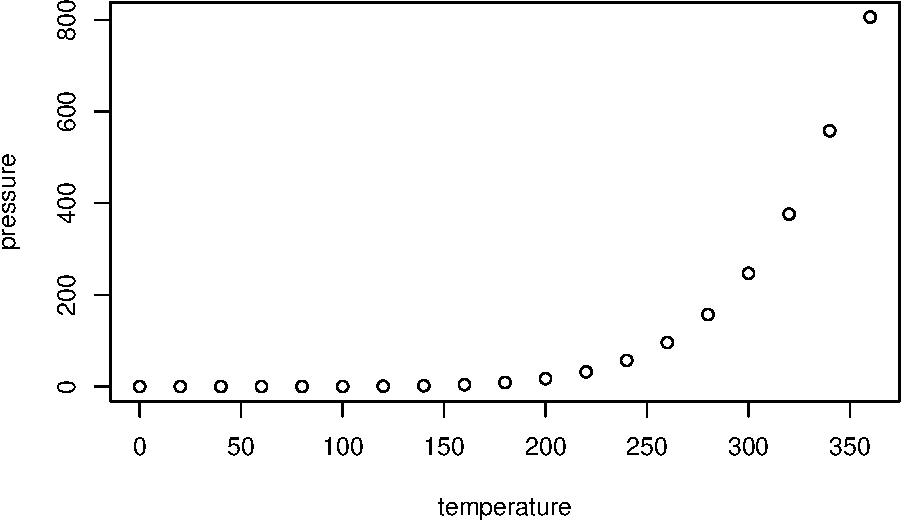
\includegraphics{thesis_files/figure-latex/pressure-1.pdf}

  Note that the \texttt{echo=FALSE} parameter was added to the code chunk to prevent printing of the \textbf{R} code that generated the plot. There are plenty of other ways to add chunk options. More information is available at \url{http://yihui.name/knitr/options/}.

  Another useful chunk option is the setting of \texttt{cache=TRUE} as you see here. If document rendering becomes time consuming due to long computations or plots that are expensive to generate you can use knitr caching to improve performance. Later in this file, you'll see a way to reference plots created in \textbf{R} or external figures.

  \hypertarget{loading-and-exploring-data}{%
  \section{Loading and exploring data}\label{loading-and-exploring-data}}

  Included in this template is a file called \texttt{flights.csv}. This file includes a subset of the larger dataset of information about all flights that departed from Seattle and Portland in 2014. More information about this dataset and its \textbf{R} package is available at \url{http://github.com/ismayc/pnwflights14}. This subset includes only Portland flights and only rows that were complete with no missing values. Merges were also done with the \texttt{airports} and \texttt{airlines} data sets in the \texttt{pnwflights14} package to get more descriptive airport and airline names.

  Testing citation ({\textbf{???}}). Or it can be ({\textbf{???}}).

  We can load in this data set using the following command:

  \hypertarget{additional-resources}{%
  \section{Additional resources}\label{additional-resources}}
  \begin{itemize}
  \item
    \emph{Markdown} Cheatsheet - \url{https://github.com/adam-p/markdown-here/wiki/Markdown-Cheatsheet}
  \item
    \emph{R Markdown} Reference Guide - \url{https://www.rstudio.com/wp-content/uploads/2015/03/rmarkdown-reference.pdf}
  \item
    Introduction to \texttt{dplyr} - \url{https://cran.rstudio.com/web/packages/dplyr/vignettes/introduction.html}
  \item
    \texttt{ggplot2} Documentation - \url{http://docs.ggplot2.org/current/}
  \end{itemize}
  \hypertarget{conclusion}{%
  \chapter*{Conclusion}\label{conclusion}}
  \addcontentsline{toc}{chapter}{Conclusion}

  If we don't want Conclusion to have a chapter number next to it, we can add the \texttt{\{-\}} attribute.

  \textbf{More info}

  And here's some other random info: the first paragraph after a chapter title or section head \emph{shouldn't be} indented, because indents are to tell the reader that you're starting a new paragraph. Since that's obvious after a chapter or section title, proper typesetting doesn't add an indent there.

  \backmatter
  \bibliographystyle{$biblio-style$}
  \bibliography{thesis}

  \markboth{References}{References}

  \noindent

  \setlength{\parindent}{-0.20in}
  \setlength{\leftskip}{0.20in}
  \setlength{\parskip}{8pt}

  \hypertarget{refs}{}
  \begin{cslreferences}
  \leavevmode\hypertarget{ref-book-example}{}%
  Abraham, R., J. E. Marsden, and T. Ratiu. 1988. \emph{Manifolds, Tensor Analysis, and Applications}. 2nd ed. New York: Springer-Verlag.

  \leavevmode\hypertarget{ref-techreport-exampleIn}{}%
  Garret, D. A. 1977. ``The Microscopic Detection of Corrosion in Aluminum Aircraft Structures with Thermal Neutron Beams and Film Imaging Methods.'' In: Report NBSIR 78-1434. Washington, D.C.: National Bureau of Standards.

  \leavevmode\hypertarget{ref-article-example}{}%
  Iesan, D. 1996. ``Existence Theorems in the Theory of Mixtures.'' \emph{Journal of Elasticity} 42 (2): 145--63.
  \end{cslreferences}
\end{document}
